
%(BEGIN_QUESTION)
% Copyright 2007, Tony R. Kuphaldt, released under the Creative Commons Attribution License (v 1.0)
% This means you may do almost anything with this work of mine, so long as you give me proper credit

{\it Specific gravity} is defined as the ratio of densities between a particular fluid and a reference fluid.  For liquids, the reference fluid is water; for gases, the reference fluid is air.

For example, the density of olive oil is 57.3 lb/ft$^{3}$ and the density of water is 62.4 lb/ft$^{3}$.  Calculating the ratio of these two densities yields the specific gravity of olive oil: 0.918.  That is to say, the density of olive oil is 91.8\% that of water.

\vskip 10pt

A useful definition of specific gravity when performing hydrostatic pressure calculations for various liquids is the ratio of equivalent water column height to the height of a particular liquid.  Using the specific gravity of olive oil (0.918) as an example, we could say that 0.918 units of water column height will generate the same hydrostatic pressure as 1 unit of olive oil height.  The unit could be ``inches,'' ``centimeters,'' ``millimeters,'' ``cubits,'' or anything else:

$$0.918 \hbox{ unit W.C. pressure} = 1 \hbox{ unit olive oil pressure}$$

We may make a ``unity fraction'' from this equality, since we are dealing with two physically equal quantities: the amount of hydrostatic pressure generated by two vertical columns of different liquids.

$${{0.918 \hbox{ unit W.C.}} \over {1 \hbox{ unit olive oil}}} = \hbox{ unity}$$

Apply this ``unity fraction'' to the calculation of hydrostatic pressure at the bottom of a 20 foot tall storage tank filled to the top with olive oil, expressing that pressure in units of kPa.  Show how the units cancel in your calculation(s), beginning with feet of olive oil and ending in kilo-Pascals (kPa):

$$\includegraphics[width=15.5cm]{i02956x01.eps}$$

\underbar{file i02956}
%(END_QUESTION)





%(BEGIN_ANSWER)

$$\left( {{20 \hbox{ ft olive oil}} \over 1} \right)  \left({{0.918 \hbox{ ft W.C.}} \over {1 \hbox{ ft olive oil}}}\right) \left({{12 \hbox{ inches}} \over {1 \hbox{ ft}}}\right)  \left( {{6.895 \hbox{ kPa}} \over {27.6807 \hbox{ inches W.C.}}} \right) = 54.88 \hbox{ kPa}$$

%(END_ANSWER)





%(BEGIN_NOTES)

%INDEX% Measurement, level: hydrostatic pressure
%INDEX% Physics, static fluids: density and specific gravity

%(END_NOTES)


